\documentclass{article}
\pagestyle{plain}

\title{Data Prefetching Championship\\
        \large{Lab3-Advanced Memory Systems}}
\author{Ramyad Hadidi}
\date{\today}

\usepackage{graphicx}
\usepackage{amsmath}
\usepackage{hyperref}
\usepackage{listings}
\usepackage{color}
\usepackage[usenames,dvipsnames]{xcolor}

\begin{document}

\definecolor{light-blue}{RGB}{216,208,255}
\lstset{language=C++, 
	basicstyle=\fontsize{9}{9}\selectfont\ttfamily,
        keywordstyle=\color{Blue}\ttfamily,
        stringstyle=\color{Red}\ttfamily,
        commentstyle=\color{ForestGreen}\ttfamily,
        breaklines=true
	backgroundcolor=\color{light-blue}, 
	frame=single,
	numbers=left, 
	stepnumber=1,
	numberstyle=\tiny\color{Sepia},
	morekeywords={}}

\maketitle

\begin{abstract}
This is the report for Lab3 assignment for Advanced Memory Systems (ECE-7103A) taught by Moinuddin Qureshi on Spring 2015. This assignment is about data prefetching policies. The framework is provided by second data prefetching championship (DPC2). The framework has some traces and basic policies. In this assignment we will measure the performance and sensitivity to prefetching degree of these policies with provided traces. Then, we will develop an online mechanism to change these policies during execution. Finally, we will design a new policy of our own. 
\end{abstract}

\section{Introduction}
In this lab we experiment with different data prefetching policies. Simulation framework is provided by second data prefetching championship (DPC2), available on \url{http://comparch-conf.gatech.edu/dpc2/}. In this section we get familiar with policies, workloads, system configuration and how to execute simulation. In the following sections, first we measure the performance of these four prefetchers and compare them with no prefetching performance. Second, we will change the degree of provided prefetchers and measure the sensitivity of each workload to aggressiveness of the prefetcher.

\subsection{Included Policies}
Provided framework has these three included policies:
\begin{description}
 \item [Next Line Prefetcher]: A simple prefetcher which will prefetch next address of current accessed cache line.
 \item [Program Counter Based Stride Prefetcher]: A stride prefetcher which will detect same strides coming from a single program counter and then prefetches additional lines.
 \item [Stream Prefetcher]: This prefetcher monitors a window of addresses in a page. After confirming the direction of the accesses, it prefetches additional lines.
 \item [Access Map Pattern Matching (AMPM) Prefetcher]: This prefetcher monitors a page for accesses. Then, it tries to match a pattern to the accesses. If the pattern matches, it do the prefetching. Patterns are offset prefetches with different offsets. However, this prefetcher is the lite version of the original AMPM prefetcher which has a larger monitoring address area. 
\end{description}

\subsection{Workloads}
The framework has some short traces. For this assignment these traces will be used. They are 8 traces from SPEC CPU 2006 with almost 3~million instructions each. Here is the list of these workloads:
\begin{table}[!h]
\centering
\begin{tabular}{|| c | c ||}
\hline \hline 
gcc & GemsFDTD \\
lbm & leslie3D \\
libquantum & mcf \\
milc & omnetpp \\
\hline \hline
\end{tabular}
\caption{Workloads}
\label{table_bench}
\end{table}

\subsection{System Configurations}
Framework models a simple out-of-order core with three level of caches. The memory model consists of a 3 level cache hierarchy, with an L1 data cache, an L2 data cache, and an L3 data cache. Instruction caching is not modeled. The L1 data cache is 16KB 8-way set-associative with LRU replacement. The L2 data cache is 128KB 8-way set-associative with LRU replacement. The L3 data cache is 16-way set-associative with LRU replacement. The size of L3 cache and bus bandwidth is a configuration parameter. The L2 data cache is inclusive of the L1, and the L3 data cache is inclusive of both the L1 and L2. Prefetcher works at cache line granularity and works in the physical address space only, and is restricted from crossing 4 KB physical page boundaries. The prefetchers can only see the stream of L1 cache misses / L2 cache reads (including those L2 reads caused by an L1 write miss). In other words, the prefetcher lives at the L2 level of cache. For more detailed description look at \url{http://comparch-conf.gatech.edu/dpc2/simulation_infrastructure.html}.

\subsection{Framework}
Prefetchers code are in \verb+example_prefetchers+ directory. The simulator code is provided as a library in \verb+lib+ directory. To compile an executable of the simulator below command is used:
\footnotesize\begin{verbatim}
 gcc -Wall -o dpc2sim example_prefetchers/stream_prefetcher.c lib/dpc2sim.a
\end{verbatim}\normalsize
Simulator read traces from stdin. So to execute a gzip trace:
\footnotesize\begin{verbatim}
 zcat trace.dpc.gz | ./dpc2sim
\end{verbatim}\normalsize
For easiness, I have written a python script, \verb+run.py+ to compile and execute different prefetches in \verb+example_prefetchers+ directory. Below is the help of this script:
\footnotesize\begin{verbatim}
 usage: run.py [-h] [--dryRun] [-o OUTPUTDIR] [-e [EXE [EXE ...]]] [-s]
              [-d DEGREE]

run.py

optional arguments:
  -h, --help            show this help message and exit
  --dryRun              Print out the generated script(s) instead of launching
                        jobs
  -o OUTPUTDIR, --outputDir OUTPUTDIR
                        Root directory for result files
  -e [EXE [EXE ...]], --exe [EXE [EXE ...]]
                        Executables to run
  -s, --submit          Submit Jobs to qsub
  -d DEGREE, --degree DEGREE
                        Degree of Prefetcher, for name generation
\end{verbatim}\normalsize
This script save the output of the simulator to a directory. After that, finding the corresponding performance is easy with \verb+grep+ command.


\section{Policies Performance}
Figure \ref{pic:perf} shows the performance speedups for different policies. X axis is the traces and Y axis is speedup based on IPC. Positive values shows speed up and negative values shows slow downs. AMPM is the best policy across all other policies. The online policy is my own designed mechanism to detect best policy in execution. 

\begin{figure}[h!]
  \label{pic:perf}
  \centering
    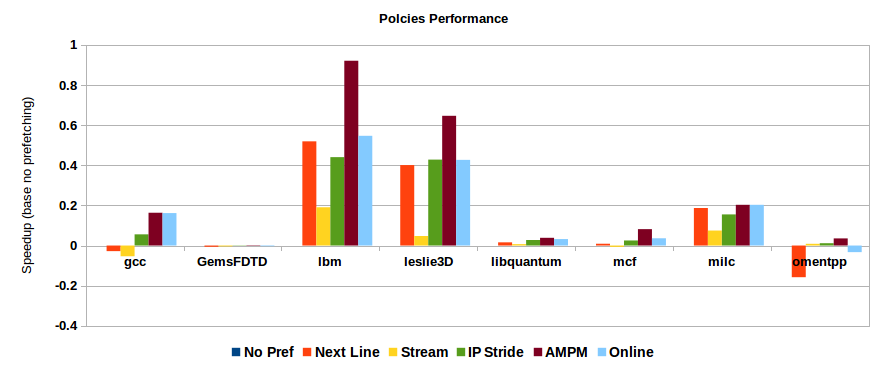
\includegraphics[width=1\textwidth]{perf.png}
    \caption{Policies Speedup in IPC - Normalized to No Prefetching}
\end{figure}

\section{Sensitivity of Workloads to Prefetcher Aggressiveness}
In this section we evaluate the sensitivity of each workload to the aggressiveness of prefetchers. Aggressiveness is defined as prefetching degree in the code. It means that how many prefetches will be done for a demand access. In following subsections we investigate this for different policies.

\subsection{Next Line}

\begin{figure}[!h]
  \label{pic:next-agg}
  \centering
    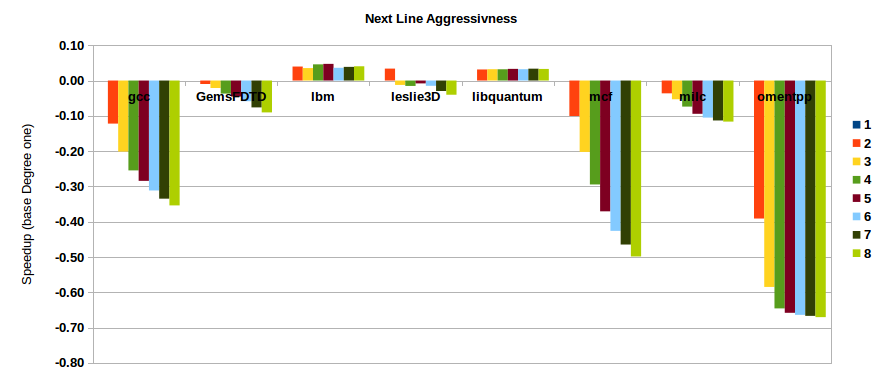
\includegraphics[width=1\textwidth]{next_agg.png}
    \caption{Next Line Policy Aggressiveness impact on Speedup - Normalized to degree one}
\end{figure}

\subsection{IP Stride}


\begin{figure}[!h]
  \label{pic:ip-agg}
  \centering
    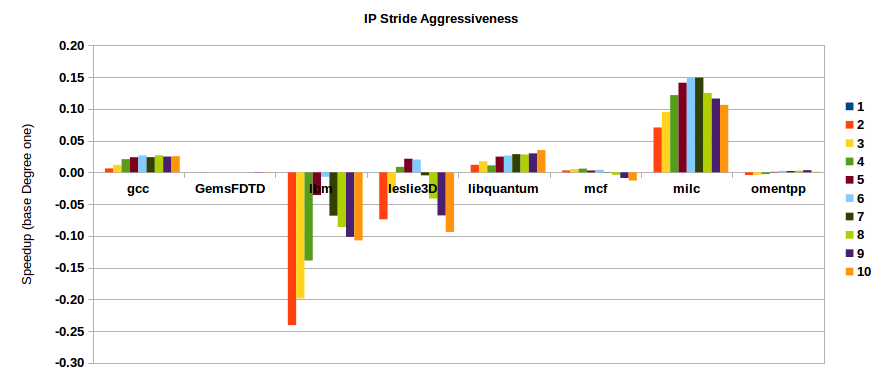
\includegraphics[width=1\textwidth]{ip_agg.png}
    \caption{IP Stride Policy Aggressiveness impact on Speedup - Normalized to degree one}
\end{figure}

\subsection{Stream}


\begin{figure}[!h]
  \label{pic:stream-agg}
  \centering
    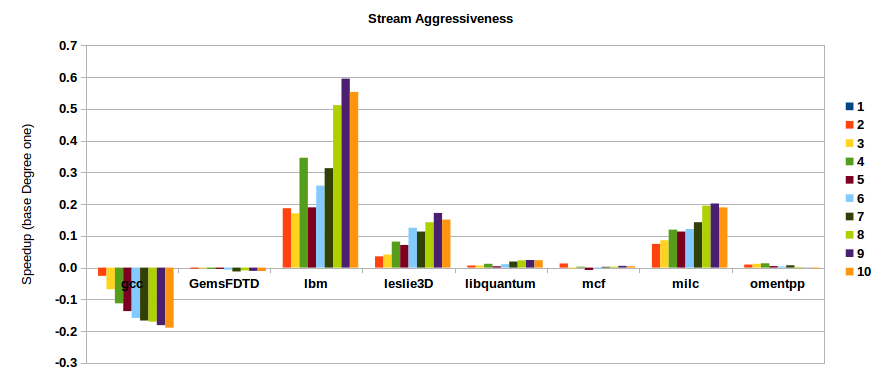
\includegraphics[width=1\textwidth]{stream_agg.png}
    \caption{Stream Policy Aggressiveness impact on Speedup - Normalized to degree one}
\end{figure}

\subsection{AMPM}

\begin{figure}[!h]
  \label{pic:ampm-agg}
  \centering
    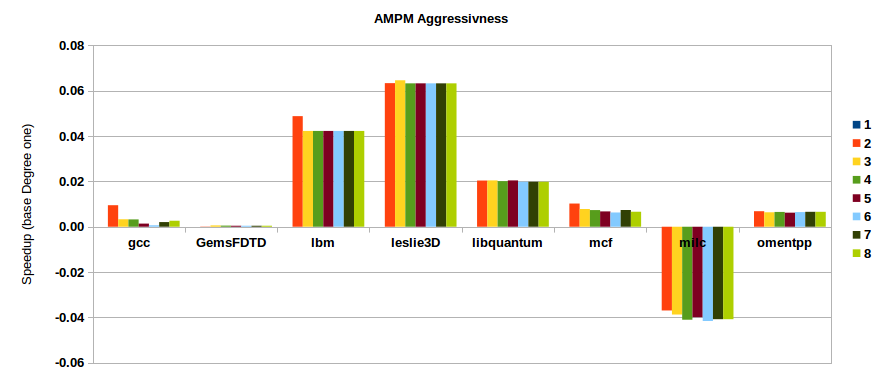
\includegraphics[width=1\textwidth]{ampm_agg.png}
    \caption{AMPM Policy Aggressiveness impact on Speedup - Normalized to degree one}
\end{figure}

\section{Online Prefetching Mechanism}

\section{Proposed Improved Prefetcher}

% \clearpage
% 
% \bibliographystyle{plain}
% \bibliography{refrences}
\end{document}
